\section{System Design / Architecture of Proposed Work}

\subsection{Architectural Overview}
SIGS-RS is structured as an event-driven, multi-stage ingestion and security gateway. The system decouples network ingress from persistent database writes through asynchronous in-memory queues and worker tasks, ensuring that edge socket latency remains unaffected by database operations.

\begin{figure}[H]
\centering
\begin{tikzpicture}[
    node distance=1.2cm and 1.0cm,
    box/.style={draw, rounded corners, minimum width=2.6cm, minimum height=0.9cm, align=center, font=\footnotesize\bfseries, fill=blue!5},
    storage/.style={draw, cylinder, shape border rotate=90, aspect=0.25, minimum width=2.4cm, minimum height=1.2cm, align=center, font=\footnotesize\bfseries, fill=orange!10},
    gate/.style={draw, rounded corners, minimum width=2.8cm, minimum height=0.9cm, align=center, font=\footnotesize\bfseries, fill=red!10},
    arrow/.style={->, >=stealth, thick},
    dashedarrow/.style={->, >=stealth, dashed, thick, red!70!black}
]

% Producers
\node[box, fill=gray!10] (sim) {Virtual Sensor Grid\\(Simulator CLI)};

% Ingestion
\node[box, right=1.2cm of sim, yshift=0.8cm] (mqtt) {MQTT Ingestion\\(Port 8883 / TLS)};
\node[box, right=1.2cm of sim, yshift=-0.8cm] (http) {HTTP REST Ingestion\\(POST /telemetry)};

% Queue
\node[box, fill=yellow!15, right=1.2cm of mqtt, yshift=-0.8cm] (queue) {IngestionQueue\\(asyncio.Queue)};

% Middleware Stage 1 & 2
\node[gate, right=1.2cm of queue, yshift=0.8cm] (inspector) {Stage 1: Inspector\\• Sliding Window\\• Physical Bounds};
\node[gate, fill=green!10, right=1.2cm of inspector] (anonymizer) {Stage 2: Anonymizer\\• PII Stripping\\• Fail-Secure Gate};

% Persistence Guard & Storage
\node[box, fill=purple!10, below=1.2cm of anonymizer] (cb) {Circuit Breaker\\(Latency $< 2000$ ms)};
\node[storage, left=1.2cm of cb] (db) {TimescaleDB\\sanitized\_readings};
\node[storage, fill=red!10, below=1.2cm of inspector] (audit) {Security Audit Sink\\audit.security\_log};

% Connections
\draw[arrow] (sim) |- (mqtt);
\draw[arrow] (sim) |- (http);
\draw[arrow] (mqtt) -| (queue);
\draw[arrow] (http) -| (queue);
\draw[arrow] (queue) |- (inspector);
\draw[arrow] (inspector) -- node[above, font=\scriptsize] {Verified} (anonymizer);
\draw[dashedarrow] (inspector) -- node[left, font=\scriptsize] {Drop Anomaly} (audit);
\draw[arrow] (anonymizer) -- (cb);
\draw[arrow] (cb) -- (db);
\draw[dashedarrow] (cb) -| (audit);

\end{tikzpicture}
\caption{SIGS-RS System Architecture Topology (Diagram 1)}
\label{fig:system_architecture}
\end{figure}

\subsection{Ingestion Transport and Buffer Decoupling}
The gateway exposes two distinct network ingestion transports:
\begin{enumerate}[label=(\alph*)]
    \item \textbf{MQTT Subscriber (\texttt{mqtt\_sub.py}):} An asynchronous client powered by \texttt{aiomqtt}. Connects over TLS 1.2+ on port 8883, subscribes to topic wildcard \texttt{telemetry/\#}, and deserializes incoming payloads.
    \item \textbf{HTTP Ingestion Router (\texttt{http\_ingest.py}):} FastAPI endpoint exposing \texttt{POST /api/v1/telemetry}.
\end{enumerate}

Both transports execute low-latency size gating ($\le 512$~KB) and Pydantic schema parsing before placing packets into the shared \texttt{IngestionQueue}. Ingestion handlers return an HTTP 202 \texttt{Accepted} response immediately, ensuring sensor threads never block waiting for sequential middleware execution.

\subsection{Telemetry Processing Sequence}
Figure~\ref{fig:telemetry_sequence} illustrates the step-by-step processing lifecycle for each telemetry packet, highlighting the drop and audit branches.

\begin{figure}[H]
\centering
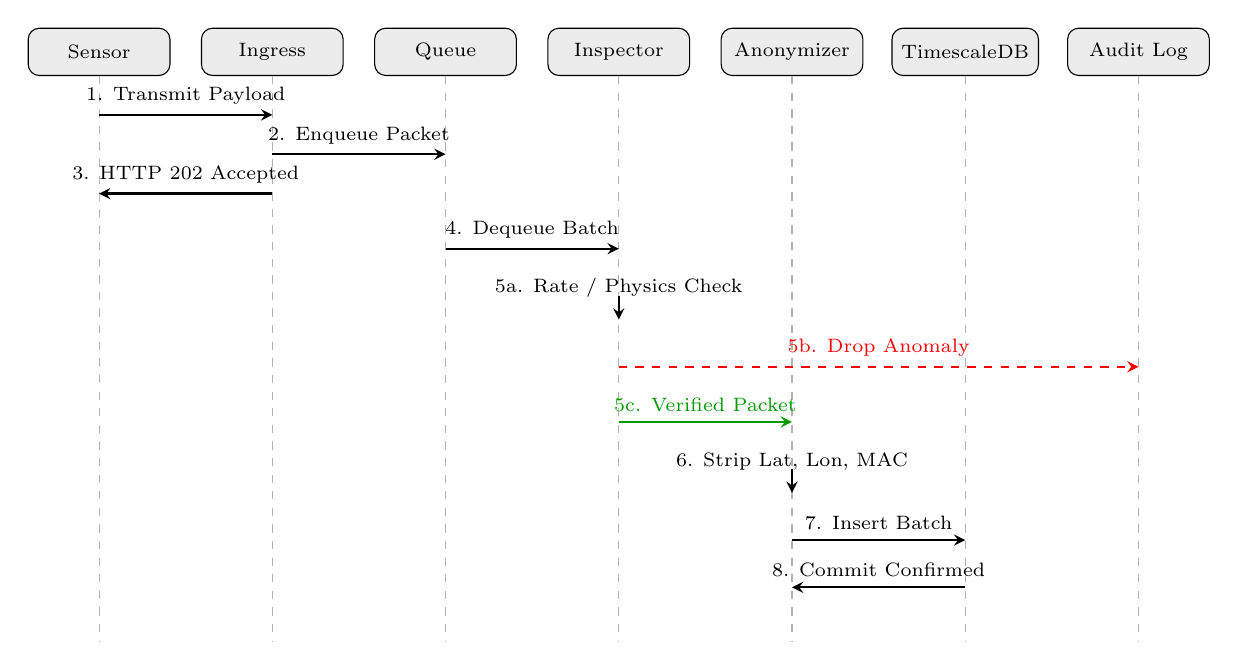
\begin{tikzpicture}[
    font=\scriptsize,
    actor/.style={draw, rounded corners, minimum width=1.8cm, minimum height=0.6cm, align=center, fill=gray!15},
    line/.style={draw, dashed, gray!60},
    msg/.style={->, >=stealth, thick},
    altbox/.style={draw, dotted, thick, inner sep=4pt}
]

% Lifelines
\node[actor] (sensor) at (0, 0) {Sensor};
\node[actor] (ingest) at (2.2, 0) {Ingress};
\node[actor] (queue) at (4.4, 0) {Queue};
\node[actor] (inspector) at (6.6, 0) {Inspector};
\node[actor] (anon) at (8.8, 0) {Anonymizer};
\node[actor] (db) at (11.0, 0) {TimescaleDB};
\node[actor] (audit) at (13.2, 0) {Audit Log};

\draw[line] (sensor) -- (0, -7.5);
\draw[line] (ingest) -- (2.2, -7.5);
\draw[line] (queue) -- (4.4, -7.5);
\draw[line] (inspector) -- (6.6, -7.5);
\draw[line] (anon) -- (8.8, -7.5);
\draw[line] (db) -- (11.0, -7.5);
\draw[line] (audit) -- (13.2, -7.5);

% Messages
\draw[msg] (0, -0.8) -- node[above] {1. Transmit Payload} (2.2, -0.8);
\draw[msg] (2.2, -1.3) -- node[above] {2. Enqueue Packet} (4.4, -1.3);
\draw[msg] (2.2, -1.8) -- node[above] {3. HTTP 202 Accepted} (0, -1.8);

\draw[msg] (4.4, -2.5) -- node[above] {4. Dequeue Batch} (6.6, -2.5);
\draw[msg] (6.6, -3.1) -- node[above] {5a. Rate / Physics Check} (6.6, -3.4);

% Anomaly Drop branch
\draw[msg, dashed, red] (6.6, -4.0) -- node[above] {5b. Drop Anomaly} (13.2, -4.0);

% Verified branch
\draw[msg, green!60!black] (6.6, -4.7) -- node[above] {5c. Verified Packet} (8.8, -4.7);
\draw[msg] (8.8, -5.3) -- node[above] {6. Strip Lat, Lon, MAC} (8.8, -5.6);
\draw[msg] (8.8, -6.2) -- node[above] {7. Insert Batch} (11.0, -6.2);
\draw[msg] (11.0, -6.8) -- node[above] {8. Commit Confirmed} (8.8, -6.8);

\end{tikzpicture}
\caption{Telemetry Processing Sequence and Drop Paths (Diagram 2)}
\label{fig:telemetry_sequence}
\end{figure}

\subsection{Concurrency Lifecycle and Background Coroutines}
The application lifespan manager (\texttt{lifespan} in \texttt{src/sigs\_rs/main.py}) coordinates four concurrent background coroutines:
\begin{enumerate}[label=\textbf{\arabic*.}]
    \item \textbf{\texttt{middleware-pipeline}:} Continuously drains batches of up to 100 packets from \texttt{IngestionQueue} every 50~ms, coordinates Inspector and Anonymizer execution, and submits sanitized batches to the repository pool.
    \item \textbf{\texttt{mqtt-subscriber}:} Maintains a resilient, reconnecting socket connection to the external MQTT broker, decoding packets and placing them on the queue.
    \item \textbf{\texttt{sliding-window-cleanup}:} Periodically sweeps memory to prune stale sensor timestamp deques older than the 10-second window (default interval: 60~seconds), preventing slow memory growth.
    \item \textbf{\texttt{compliance-sync}:} Executes a 1.0-second polling loop against the \texttt{config.middleware\_settings} table to synchronize regulatory compliance lockouts (SRS BR-3) across distributed gateway replicas.
\end{enumerate}

\subsection{Fail-Closed State Transitions}
In accordance with high-assurance security engineering, SIGS-RS implements a fail-closed policy. If the \texttt{middleware-pipeline} task encounters an unhandled exception, a database connectivity failure occurs during compliance checks, or the persistence circuit breaker remains open, the gateway sets its internal \texttt{fail\_closed = True} flag. In this state:
\begin{itemize}
    \item The \texttt{/health} probe immediately returns HTTP 503 \texttt{Service Unavailable}.
    \item Incoming HTTP telemetry is refused with HTTP 503.
    \item The MQTT subscriber ceases enqueuing messages, preventing queue growth.
    \item In Kubernetes, this probe failure triggers container restart within 15 to 30 seconds (SRS REQ-QA-1).
\end{itemize}
